\documentclass[oneside]{report}
\usepackage[T1]{fontenc}
\usepackage[utf8]{inputenc}
\usepackage[frenchb]{babel}
\usepackage{graphicx}
\usepackage[margin=2cm]{geometry}
\usepackage{fancyhdr}
\usepackage{changepage}
\usepackage{etoolbox}
\usepackage{xcolor}
\usepackage{titlesec}

\titleformat{\chapter}[display]
{\normalfont\huge\bfseries}{}{20pt}{\Huge}

\titlespacing*{\chapter}{0pt}{0pt}{0pt}
\graphicspath{ {images/} }


\author{Nathan JANCZEWSKI, Léo BERGEROT, Loic HUSSON, Youness LOUCIF,\\ Alexandre QUILLET, Jonathan PAUGOIS }

\usepackage{etoolbox}
\patchcmd{\chapter}{plain}{fancy}{}{}

\newcommand{\writecol}[1] {
	\subitem{\textcolor[HTML]{#1}{\# #1}}
}

\newcommand{\indentunder}{1.5cm}
\begin{document}
	\begin{titlepage}
		\centering		
		
\includegraphics[scale=2]{logo}
		\vspace{5cm}
		{\par\scshape\Huge Cahier des charges \par}
		\vspace{0.5cm}
		{\par\scshape\Large Site web pour l'Université Pan Africaine\par}
		\vspace{10cm}
		{\par Université Pan Africaine (UPA)\par}
		{\par Site web \par}
		{\vfill}
		{\par Contact: \par}
		{\par\small Mme Zahia GUESSOUM\par}
		{\par zahia.guessoum@univ-reims.fr \par}
	\end{titlepage}		

\pagestyle{fancy}
\fancyhf{}
\rhead{
\includegraphics{logo}}
\lhead{Cahier des charges}

	\tableofcontents
	
	\chapter{Présentation de l'École}
	{
		\vspace{2cm}
		\par Les instituts des Universités Pan Africaines ont pour but d’améliorer la qualité d'apprentissage des sciences et technologies.
		\vspace{1cm}
		\par C’est en 2003 à Johannesbourg lors de la première Conférence ministérielle sur l’environnement que naît l’idée de créer un réseau destiné à promouvoir et à faciliter la mobilité des étudiants comme des enseignants, harmoniser les programmes universitaires, répondre aux défis auxquels le continent africain devra faire face et améliorer l’attractivité des études en Afrique.
		\vspace{1cm}
		\par Une des antennes de cette université est l’institut de l'Université Pan Africaine pour les Sciences de l’Eau et de l'Énergie (y compris le changement climatique) (PAUWES), institué lors de la Commission de l’Union Africaine réunie en 2008, à Tlemcen au Nord-Ouest de l’Algérie. 
		\vspace{1cm}
		\par Elle offre deux programmes d’études supérieures :
		\begin{itemize}
			\item{Master en Science de l’Énergie}
			\item{Master en Science de l’Eau}
		\end{itemize}
	}
	\chapter{Présentation du projet}
	{
		\vspace{2cm}
		\par Rendre le site web plus utile pour:
		\begin{itemize}
			\item{l'administration}
				\subitem{Inscrire les nouveaux étudiants}
				\subitem{Gérer le dossier personnel des étudiants}
				\subitem{Accéder à la base de données de tous les étudiants}
				\subitem{Mettre à jour les emplois du temps}
				\subitem{Relever les absences des étudiants}
			\item{les étudiants}
				\subitem{Accéder en ligne aux cours}
				\subitem{Accéder à l'emploi du temps personnel}
				\subitem{Consulter la messagerie}
				\subitem{Modifier les données personnelles}
				\subitem{Consulter les notes}
			\item{les enseignants}
				\subitem{Déposer les cours en ligne}
				\subitem{Consulter la messagerie}
				\subitem{Consulter son emploi du temps}
				\subitem{Gérer des notes}
				\subitem{Relever les absences des étudiants}
		\end{itemize}
		\vspace{1cm}
		\par\underline{Ce qui ne va pas}:
		\vspace{.5cm}
		\begin{adjustwidth}{\indentunder}{}
		\begin{itemize}
			\item Le site actuel est très utile à but informatif, mais ne permet aucune gestion de l'antenne algérienne.
			\item Il n'offre aucune plus-value aux étudiants suivants déjà les cours à l'université, et encore moins aux professeurs.
			\item Il y a deux carroussels présents sur toutes les pages prenant une place considérable, contraignant ainsi l'utilisateur à descendre sur la page.
			\item Le comportement de ceux-ci est très aléatoire.
			\item La présence de deux menus porte à confusion.
			\item Pas d'attribut ALT sur les images.
			\item Certaines pages ne sont pas bien classées (Welcome dans About par exemple)
		\end{itemize}
		\end{adjustwidth}
	\vspace{1cm}
	\par\underline{Ce qui va}:
		\vspace{.5cm}
		\begin{adjustwidth}{\indentunder}{}
		\begin{itemize}
			\item L'utilisation du framework Bootstrap garantit une adaptabilité et le fonctionnement sur une grande variété de navigateurs.
			\item Les informations sur le sites sont correctes.
			\item Volonté de minimiser les contrastes afin de garantir un accès aux malvoyants.
		\end{itemize}
		\end{adjustwidth}
\newpage
		\section{Comité de pilotage}
		{
			\par L’équipe attitrée au projet utilise la méthode \textit{SCRUM}. Cela veut dire que le développement se découpera en sprints, période sur laquelle l’équipe planifiera les fonctionnalités qui devront être implémentées. Cette période se conclura sur une démonstration au client, lequel pourra alors vérifier le respect du cahier des charges à son gré ainsi que la validation du graphisme et du contenu.
			\vspace{.5cm}
			\par Si le client le souhaite, la validation de l’ergonomie sera effectuée en testant sur des personnes externes (hors scolarité pour la recherche d’informations, ainsi qu’étudiants et professeurs pour leur partie respective)

		}
		\section{Objectifs du site}
		{
			Le site est d’une part un site d’information à destination d’élèves souhaitant intégrer une université, afin de décrire le fonctionnement de celle-ci, et d'autre part un support de cours et communication entre étudiants et professeurs de l’université.
		}
		
		\section{Les cibles (À qui s'adresse le site ?)}
		\par Le site s'adresse aux futurs étudiants recherchant des informations sur les diverses formations, à l'administration de l'Université, aux professeurs ainsi qu'aux élèves qui auront un accès avec plus de fonctionnalités.

		\section{Contenus}
		{
			\par Le site reprendra les diverses informations accessibles sur le site actuel, qui seront retriées afin d’obtenir une ergonomie plus accessible. Il se permettra tout de même de modifier ce qui à été inclu, celui-ci se comportant comme un CMS (ou SGC, système de gestion de contenu)
		}
		\section{Langues}
		{
			\par Le site sera conçu avec un système de traduction permettant au besoin d'ajouter d'autres langues que les deux de bases qui seront Anglais et Français.
		}

		\section{Plan du site (Arborescence)}
		{
			\par L'arborescence est la suivante:\\
			\noindent\makebox[\textwidth]{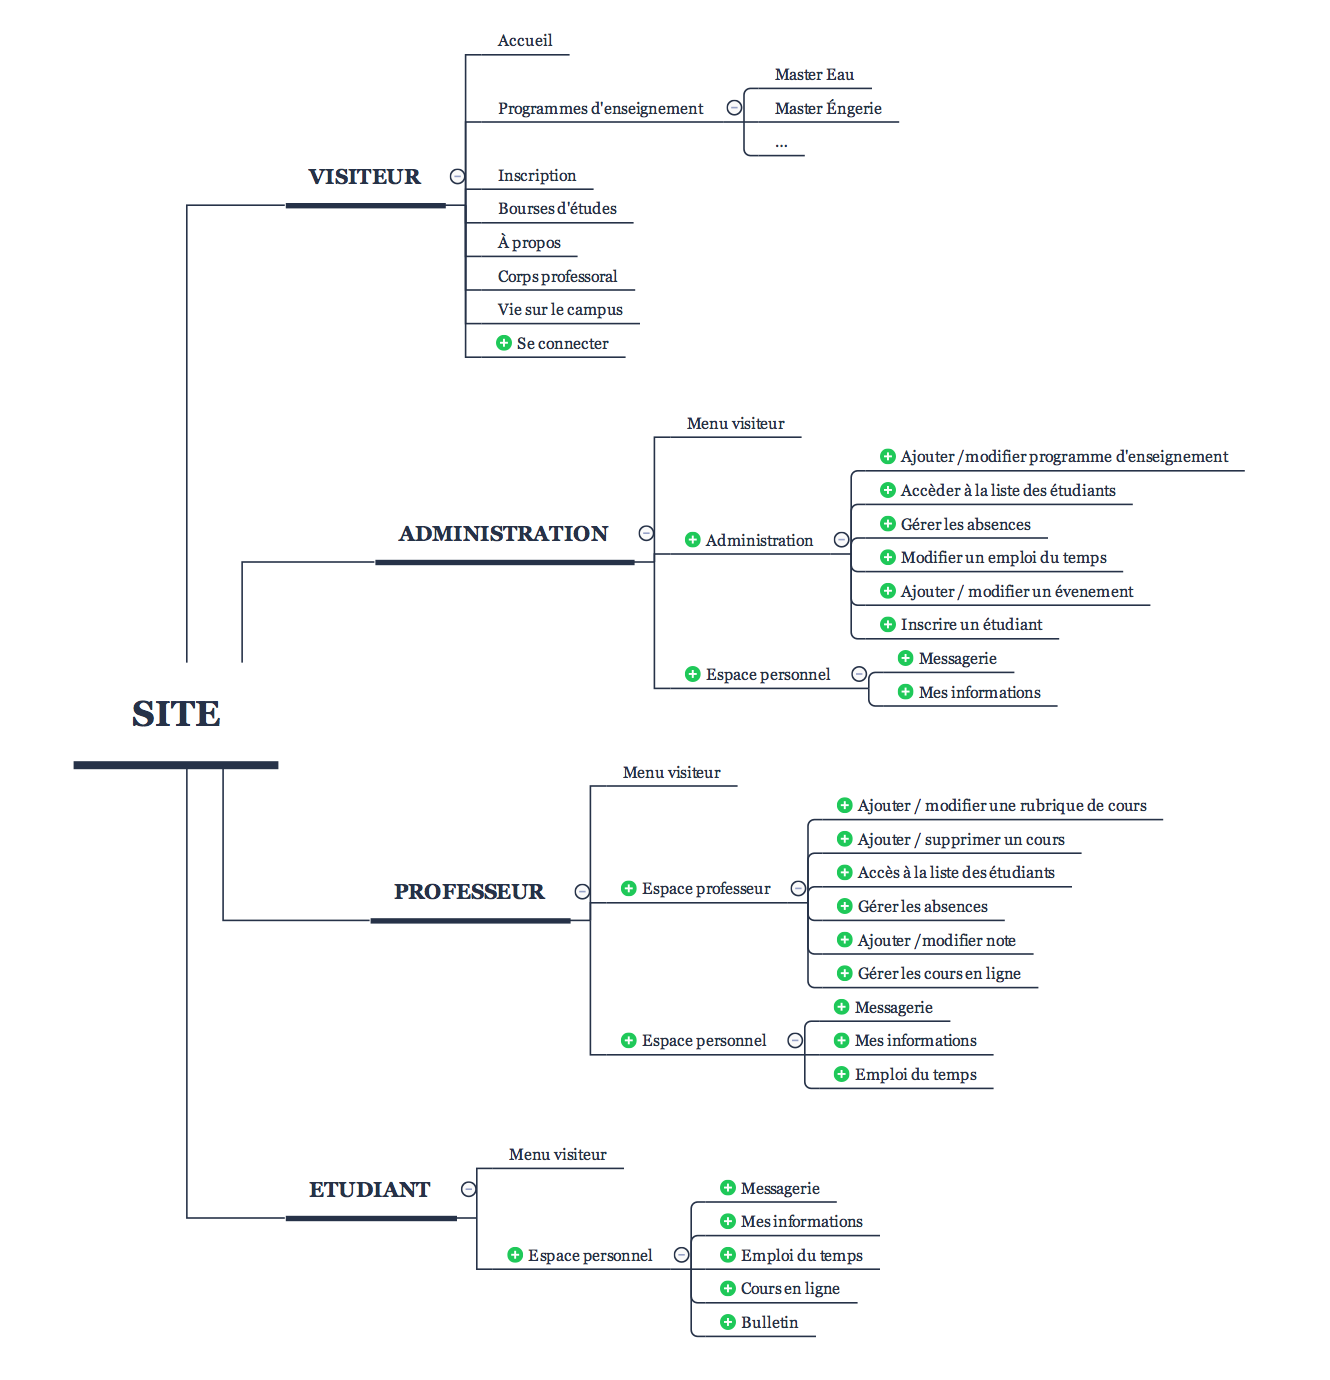
\includegraphics[scale=1]{arborescence}}
		}

		\section{Maquette du site}
		{
			\par Accès au site par un utilisateur non connecté:\\ \vspace{.5cm}
			\noindent\makebox[\textwidth]{
\includegraphics[scale=.5]{accueil}}
			\newpage
			\par Menu pour un utilisateur connecté: \\ \vspace{0.5cm}
			\noindent\makebox[\textwidth]{
\includegraphics[scale=.5]{accueil_connect_top}}
			\par Emploi du temps: \\ \vspace{0.5cm}
			\noindent\makebox[\textwidth]{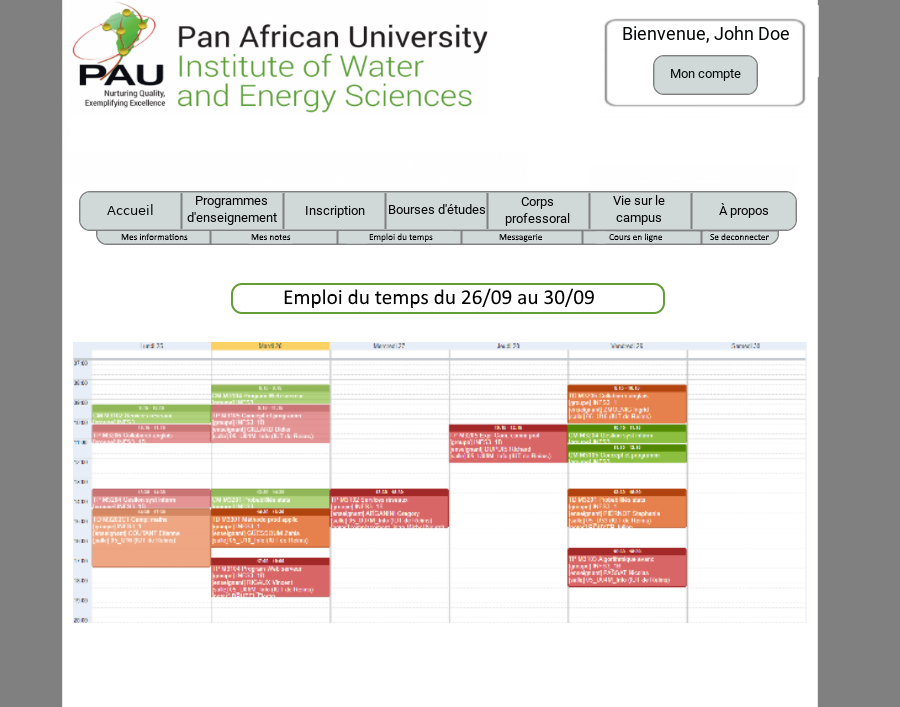
\includegraphics[scale=.5]{emploi}}
		}

	\newpage

		\section{Fonctionnalités}
		{
			\par Diagramme UML des fonctionnalités du site web:\\
			\begin{center}
				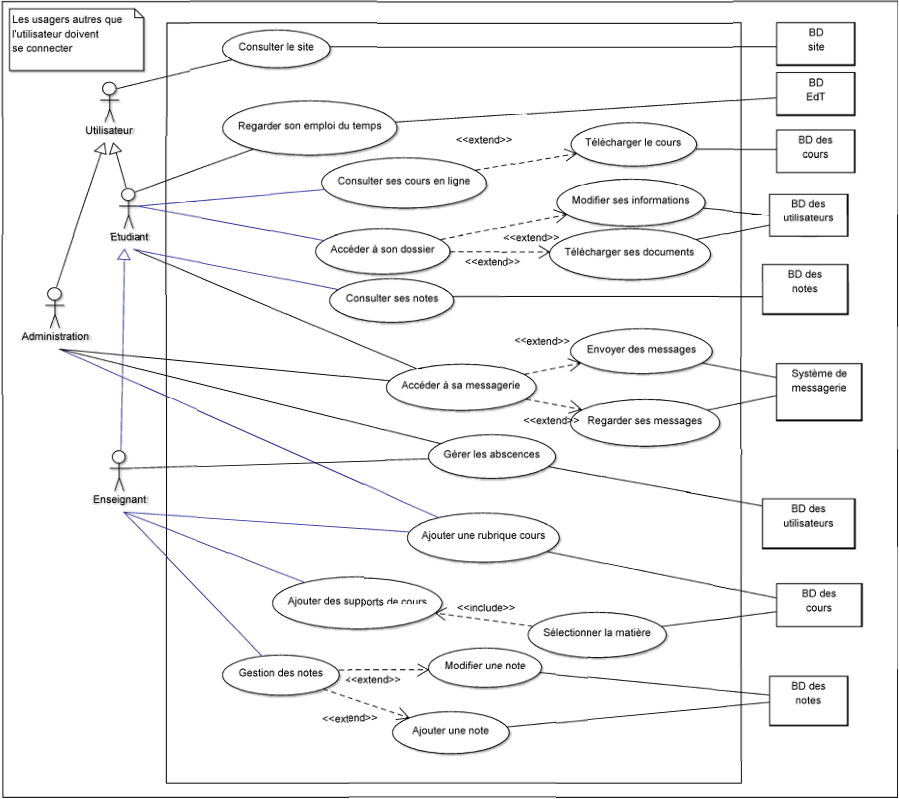
\includegraphics[scale=1.5]{uml_base}
				\\ \vspace{1cm}
				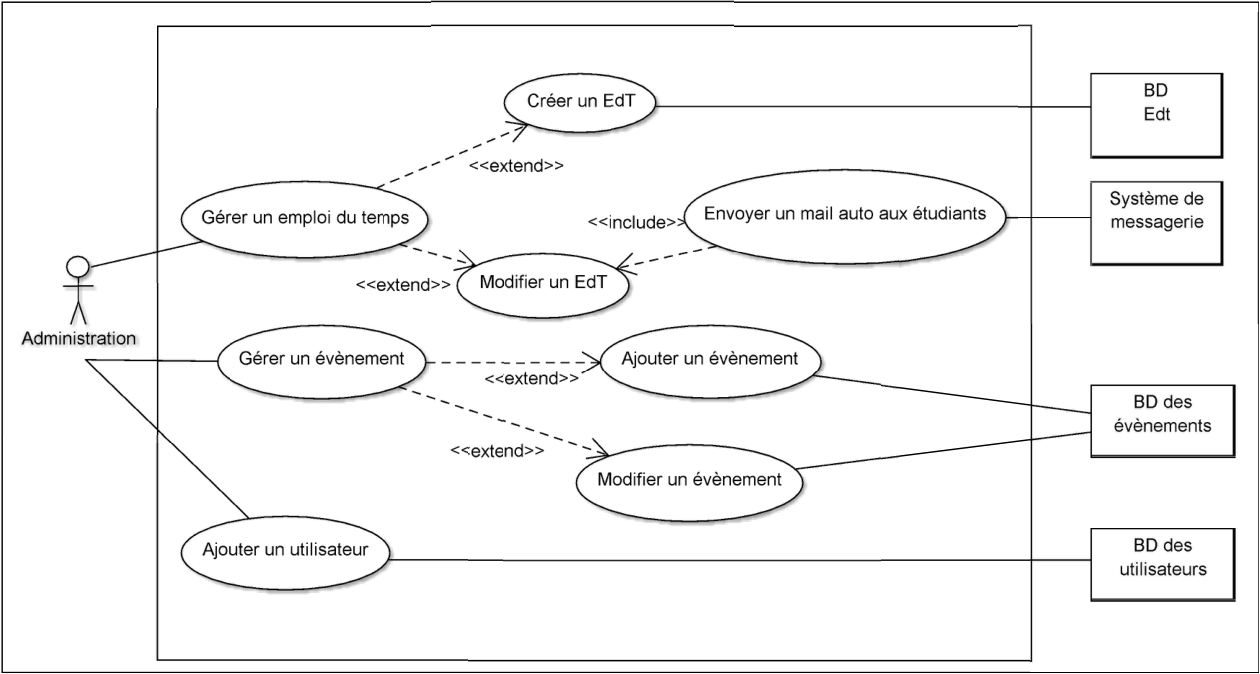
\includegraphics[scale=1.5]{uml_admin}
			\end{center}
		}
	}
	\chapter{Prestations attendues}
	{
		\section{Charte graphique}
			\begin{itemize}
				\item{Couleurs}
					\writecol{639D35}
					\writecol{040707}
					\writecol{868786}
					\writecol{005899}
					\subitem{\# FFFFFF (blanc pur)}
				\item{Typographie: Roboto Sans-Serif}
				\item{Logo}
					\subitem{
\includegraphics[scale=2]{logo}}
			\end{itemize}
		\section{Création et récupération de contenus}
		{
			\par Le contenu déjà disponible se compose de diverses photos dont les auteurs sont:
			\vspace{.5cm}
			\begin{itemize}
				\item Tlemcen University
				\item Mr Hefhaf/Tlemcen University
				\item Michael Gajo/GIZ
				\item michaeljung/Fotolia
				\item paulmz/Fotolia
				\item Piotr Pakuła/Fotolia
				\item Zurijeta/Shutterstock
				\item john michael evan potter/Shutterstock
				\item PhotoSky/Shutterstock
				\item bikeriderinlondon/Shutterstock
				\item Tyler Olson/Shutterstock
			\end{itemize}
			\vspace{.5cm}
			\par Nous nous baserons sur le contenu déjà utilisé et nous n'aurons pas besoin de contenus supplémentaires.
			\vspace{.5cm}
		}
		\section{Développement}
		\par Pour gérer correctement l’automatisation de chaque tâche, il sera nécessaire d’utiliser de la programmation orientée objet (PHP), les informations seront stockées dans une base de données (SQL).
		\par
		\begin{itemize}
			\item Gestion automatique d’ajout des formations.
			\item Gestion de la modification de l’emploi du temps avec envoi automatique d'e-mails pour prévenir les personnes.
			\item Moteur de recherche interne au site.
			\item Gestion automatique d’ajout et modification des événements (actualités).
			\item Gestion d'ajout et modification des informations personnelles (dossier étudiant, dossier professeur).
			\item Gestion d’ajout des cours en ligne et téléchargement de ceux-ci.
			\item Gestion des absences.
		\end{itemize}
		\section{Dépôt du nom de domaine et adresses mail}
		{
			\par Le nom de domaine "\textit{http://pauwes.univ-tlemcen.dz/}" étant déjà déposé, aucun coût supplémentaire ne sera à prévoir. Cependant la configuration du serveur mail peut être à prévoire en fonction de la configuration actuelle de l'hébergeur.
		}
		\section{Hébergement}
		{
			\par Le site étant destiné à remplacer l'actuel, il pourra être hébergé sur les serveurs de ce dernier.
		}
		\section{Référencement}
		{
			Le référencement devra être pris en charge par une entreprise externe.
		}
		
		\section{Mises à jour}
		{
			\par Le site étant développé comme un CMS, il a parmi ses objectifs d’être dynamique. Ainsi l’équipe administrative pourra modifier le contenu, les pages et menus depuis l’interface destinée à être simple d’utilisation.
		}
	}
	
	\chapter{Planning prévisionnel}
	{
		\par L'utilisation de la méthode agile SCRUM implique que nous recueillerons les fonctions essentiel à partir du cahier des charges et des users stories, par conséquent nous écrirons des backlogs du produit (liste des fonctionnalités) qui seront classés par priorité, permettant de définir l'ordre de réalisation et ensuite les sprints serons réalisés avec toute l'équipe de développement en décidant du sous-ensemble qui sera à réaliser à chaque fois.
	}

	\chapter{Budget}
	{
		\par Étant un projet universitaire, aucun budget n'est alloué à la crération du site web.
	}
\end{document}
